\colorlet{punct}{red!60!black}
\definecolor{background}{HTML}{EEEEEE}
\definecolor{delim}{RGB}{20,105,176}
\colorlet{numb}{magenta!60!black}

\Chapter{Tervezés}

A fejezet bemutatja az alkalmazás kinézetének, adatmodelljének és az API-jának a megtervezését.

\Section{Kinézet}

A kinézetet játékos, egyszerű és átláthatóra szeretném elkészíteni, valamint mindenhol vidám ikonokat és színvilágot szeretnék használni. Az oldal ikonjának \aref{fig:icon}. ábrán láthatót választottam, mivel a tesztek egy \textit{Game Boy}-ként fognak megjelenni:

\begin{figure}[h]
    \centering
    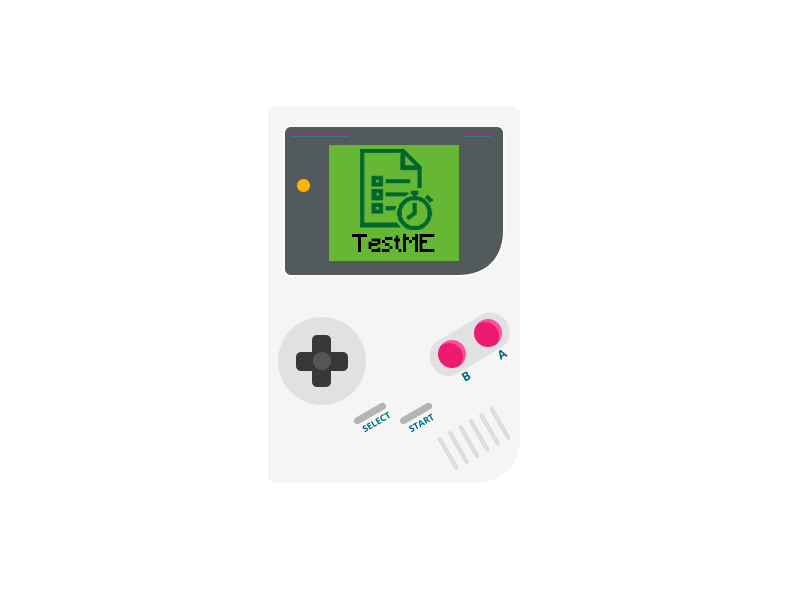
\includegraphics[height=8cm]{images/gameboy.png}
    \caption{Az alkalmazás ikonja}
    \label{fig:icon}
\end{figure}

Minden grafikus elemnél szeretném ha egységes lenne a kinézet, így törekszem arra, hogy hasonló stílusúak legyenek a továbbiak is. Az egyéb funkciókhoz vagy oldalakhoz társított ikonok szintén élénkek, színesek, egyszerűek és vidámak lesznek, hogy passzoljon az alkalmazáshoz. Kész ikonokkal dolgoztam, amelyeket a Flaticon nevű oldalról töltöttem le \cite{flaticon}. \newline

Az oldalon belül az elemek elrendezéséhez, stílusának beállításához \textit{Bootstrap}-et szeretnék használni ami egy olyan keretrendszer, amely segít a weboldalak gyorsabb és könnyebb megtervezésében. HTML és CSS alapú tervezősablonokat tartalmaz a tipográfiához, űrlapokat, gombokat, táblázatokat, navigációt, modelleket stb. Ez segít abban, hogy az oldalon egységes kinézetet hozhassak létre, valamit a Bootstrap CSS-je alkalmazkodik a telefonok, táblagépek és asztali számítógépek kijelzőjének felbontásához, megjelenítési képességeihez.

\Section{Az oldal felépítése}

A funkciók elrendezésének és felépítésének bemutatására képernyőterv vázlatot (magyarul drótváznak, angolul \textit{wireframe} vagy \textit{mockup}-nak is nevezzük) készítettem a \textit{MockFlow} \cite{mockflow} nevű oldalon.
Elsődlegesen azt az oldalt mutatom be amivel mindenki először találkozik a megnyitáskor, ez pedig a bejelentkezési és regisztrációs felület.

\SubSection{Bejelentkezés és regisztráció}

Bejelentkezni \prettyref{fig:login_wireframe}. ábrán látható űrlapon, email cím és jelszó megadásával lehet.

\begin{figure}[h!]
    \centering
    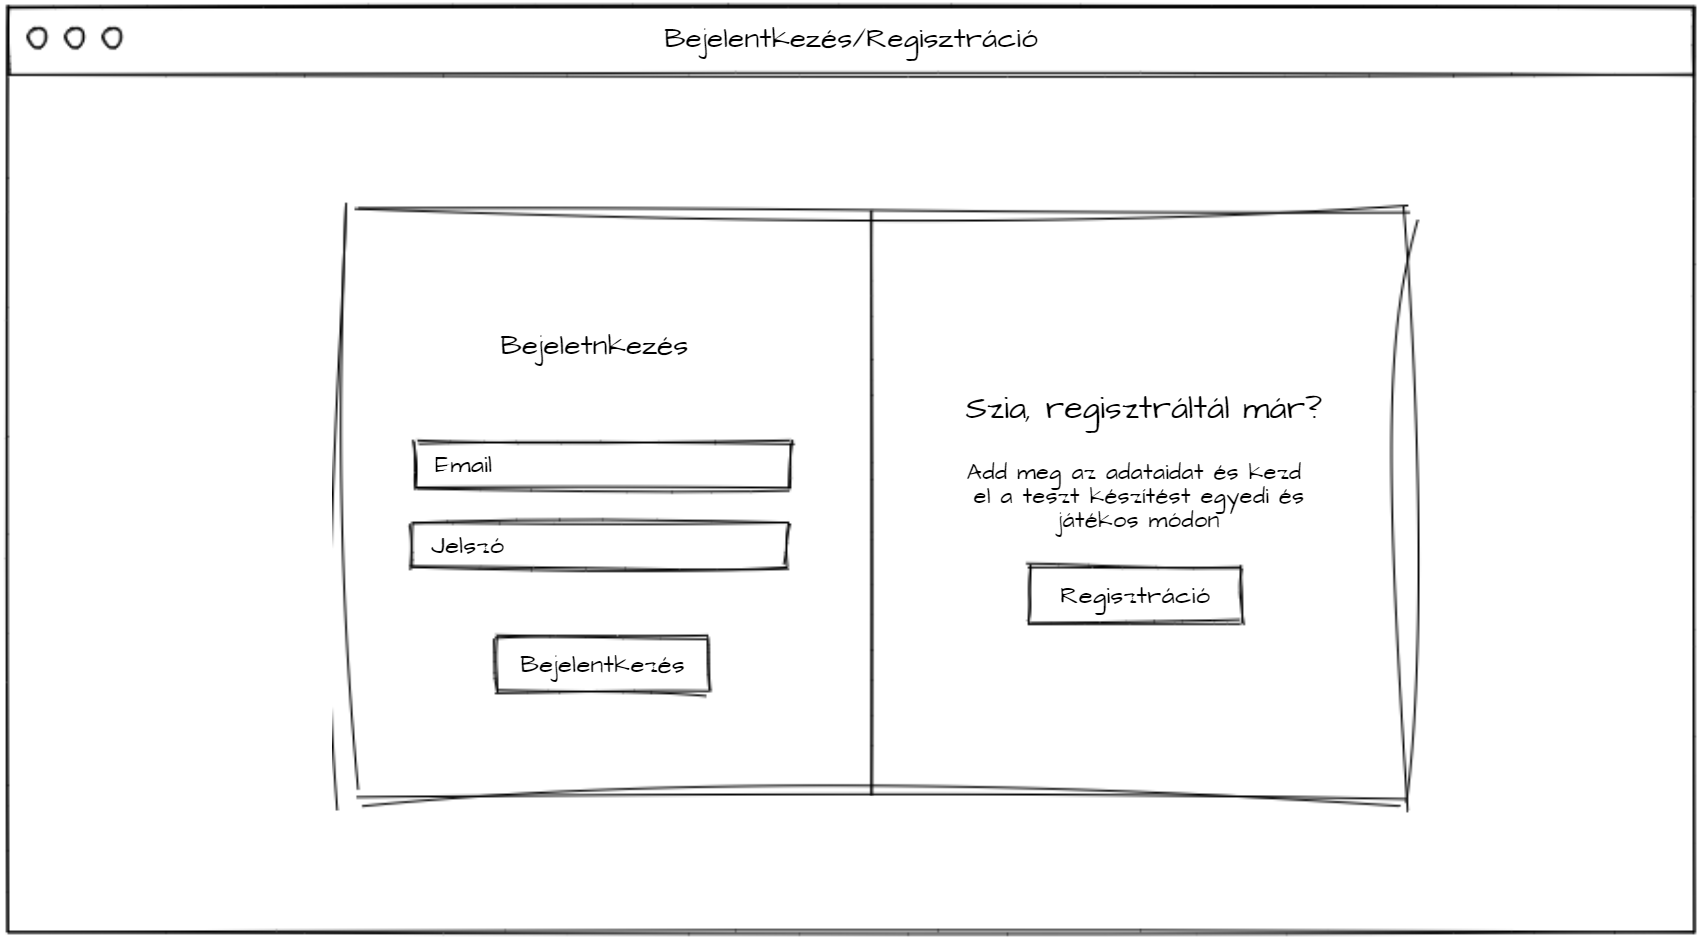
\includegraphics[width=\linewidth]{images/login_wireframe.png}
    \caption{Bejelentkezés}
    \label{fig:login_wireframe}
\end{figure}

Regisztrációkor \prettyref{fig:signin_wireframe}. ábrán látható űrlapon pedig ki kell választani, hogy tanárként vagy diákként szeretnénk regisztrálni, majd meg kell adni az alapvető adatokat.
Ezután, ha sikeresen beléptünk vagy regisztráltunk akkor hozzáférhetünk az oldalhoz.

\begin{figure}[h!]
    \centering
    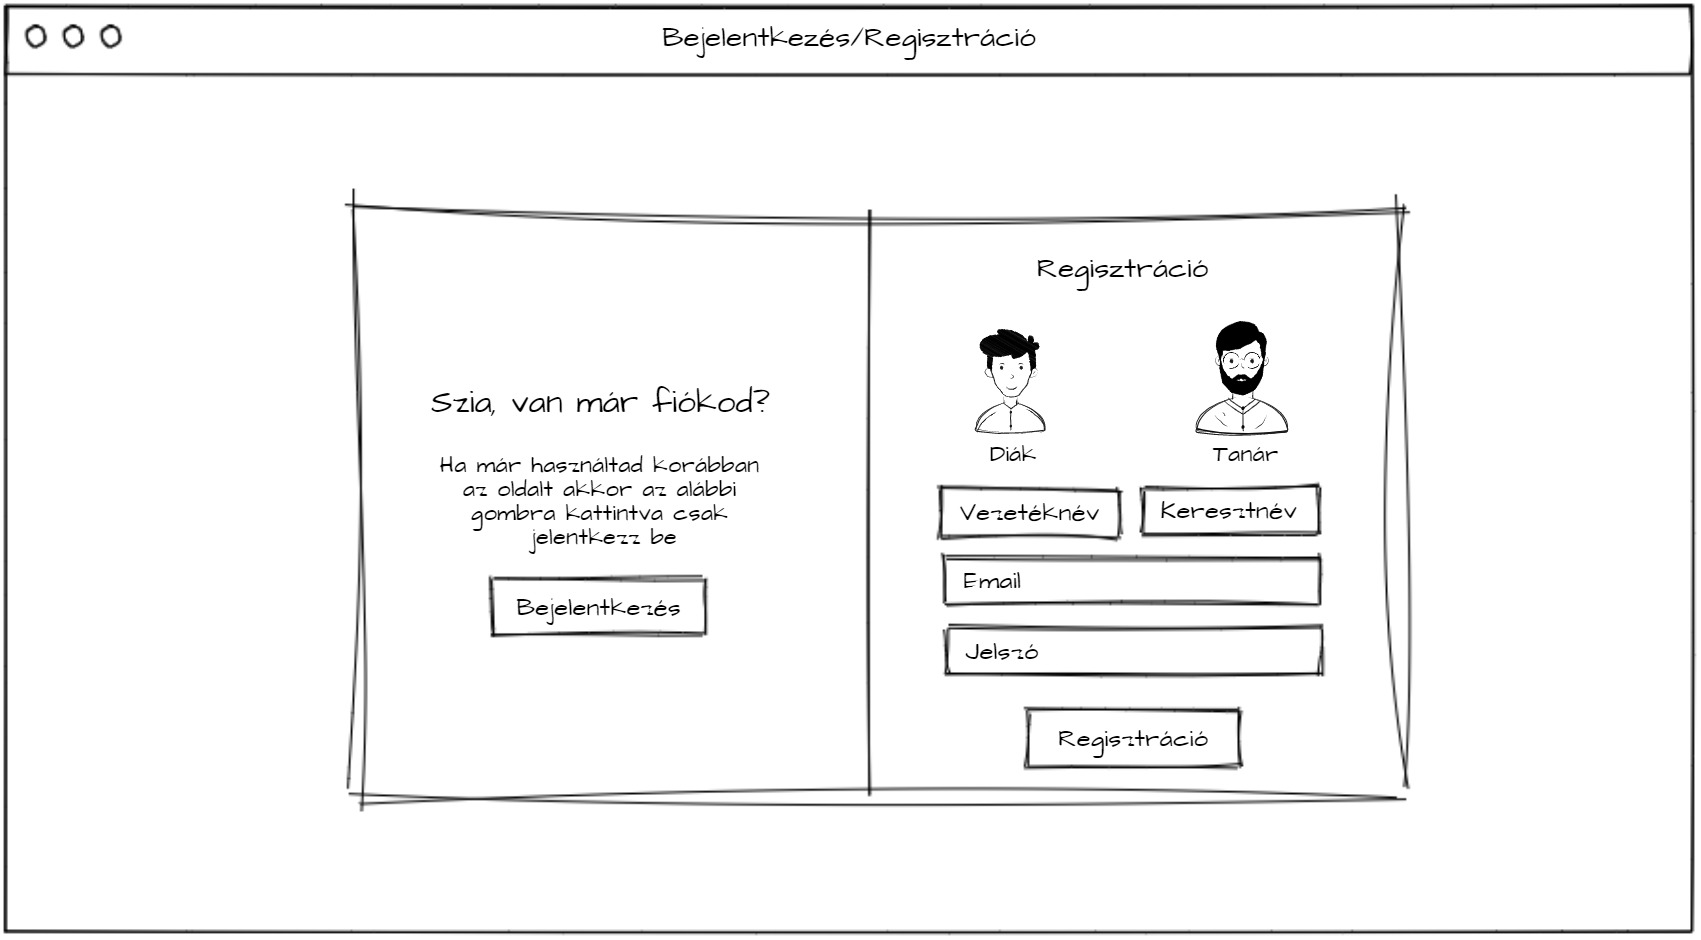
\includegraphics[width=\linewidth]{images/signin_wireframe.png}
    \caption{Regisztráció}
    \label{fig:signin_wireframe}
\end{figure}

\SubSection{Főoldal}

A főoldalon (\prettyref{fig:main_page}. ábra) láthatjuk a felhasználónevünket, hogy mennyi XP-vel rendelkezünk, hanyas szintűek vagyunk, és hogy hány darab kitöltött és kitöltetlen tesztünk van még.

\begin{figure}[h!]
    \centering
    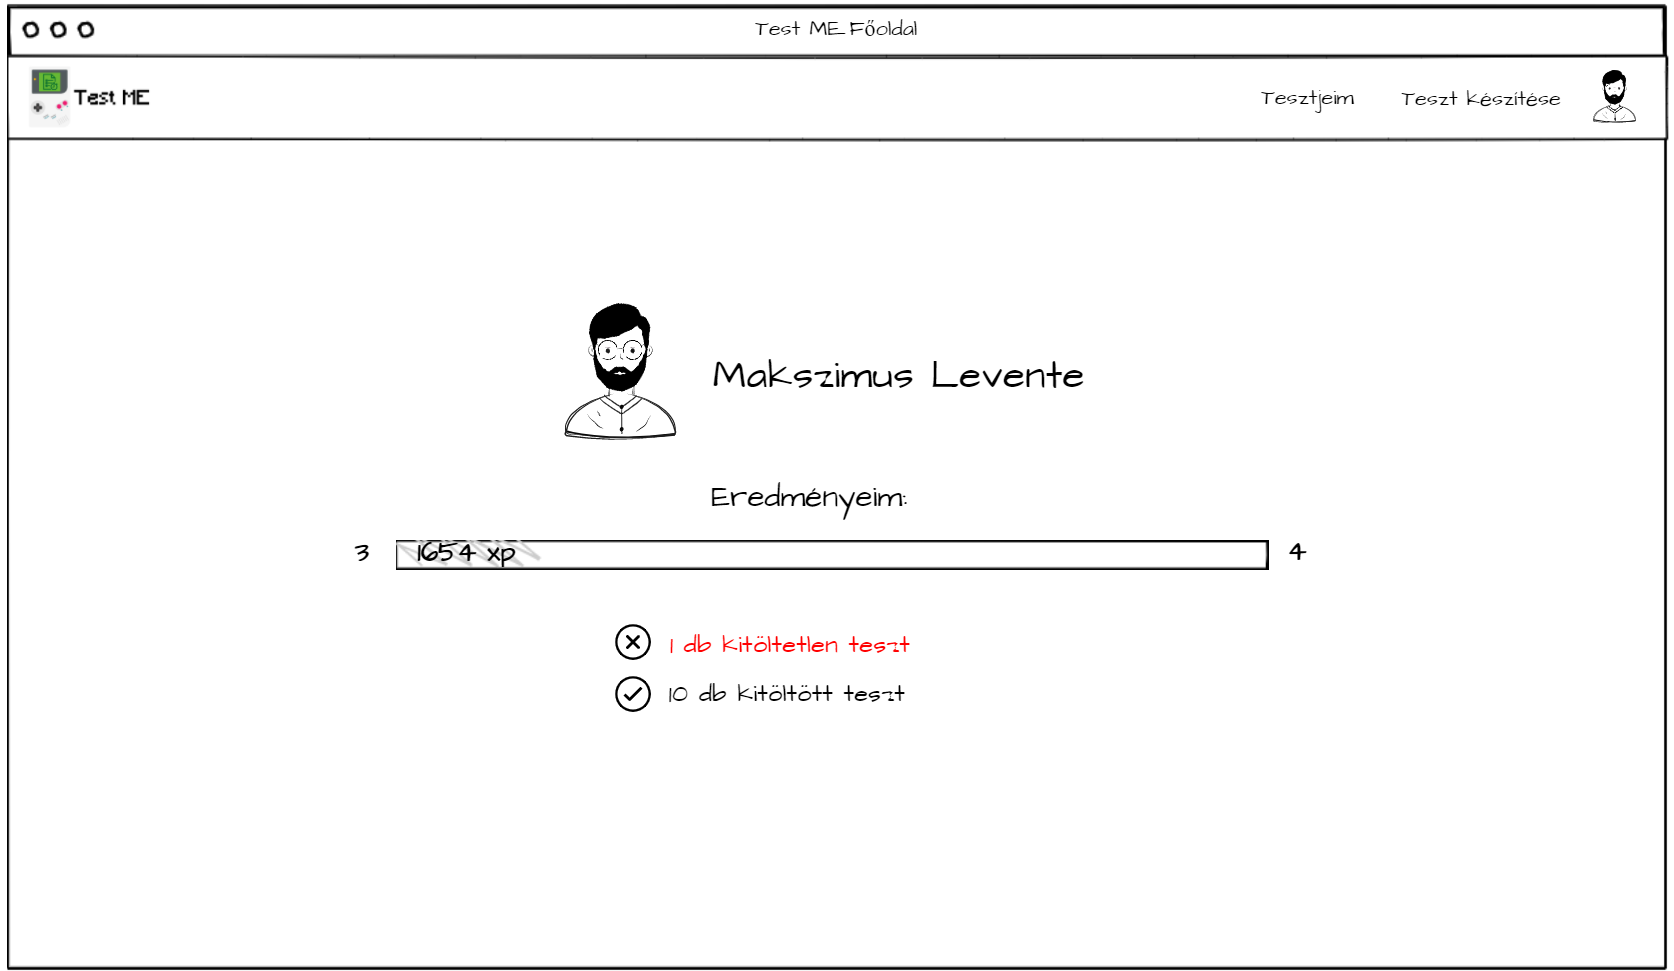
\includegraphics[width=\linewidth]{images/main_login_wireframe.png}
    \caption{Főoldal}
    \label{fig:main_page}
\end{figure}

\subsection{Teszt készítés}

\Aref{fig:new_quiz_question}. ábrán a tesztkészítési felület látható. Egy tesztnél meghatározható maga a kérdés, ideje, illetve a jutalmazása, mely XP-ként van rögzítve. A választ kiválaszthatjuk az általunk írtak közül és beállíthatjuk melyik legyen a helyes megoldás.

\begin{figure}[h!]
    \centering
    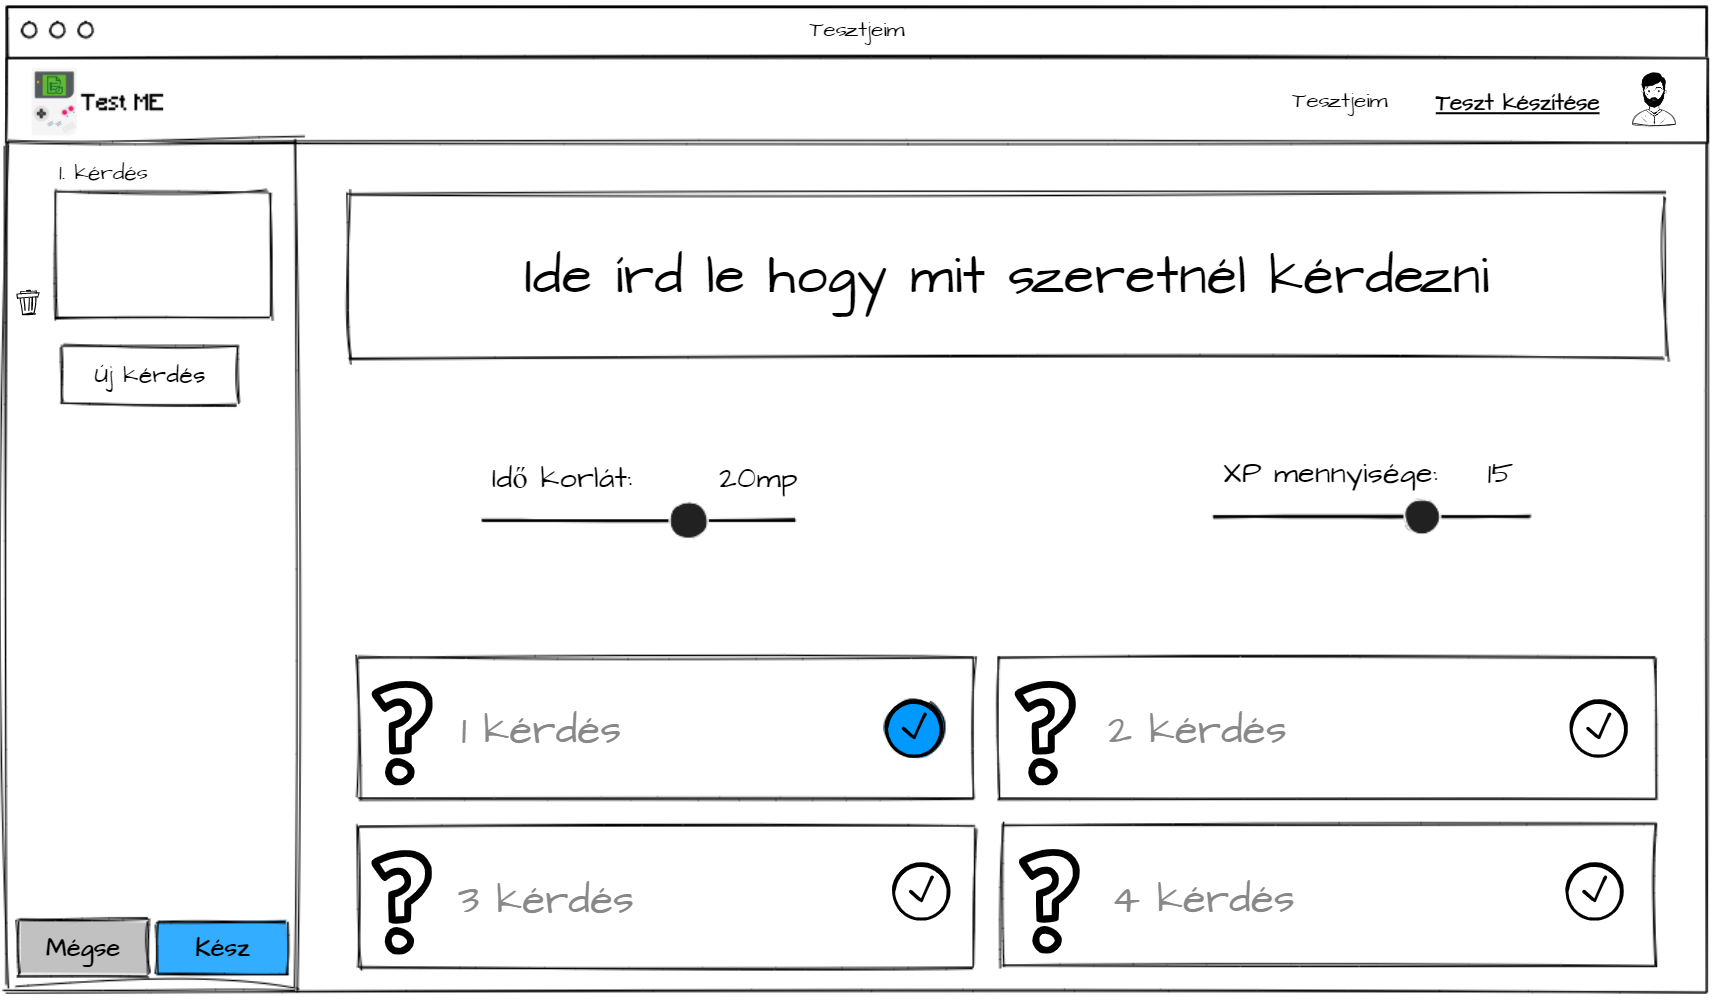
\includegraphics[width=\linewidth]{images/make_test_wireframe.png}
    \caption{Kvíz teszt készítés}
    \label{fig:new_quiz_question}
\end{figure}

Ezután ha elkészült a kérdés az ,,Új kérdés'' gomb megnyomásával lehet hozzáadni a kérdések sorába. Itt választhatunk igaz/hamis, vagy kvíz típusú alternatíva közül, hogy milyet szeretnénk feltenni (\prettyref{fig:new_question}. ábra).

\begin{figure}[h!]
    \centering
    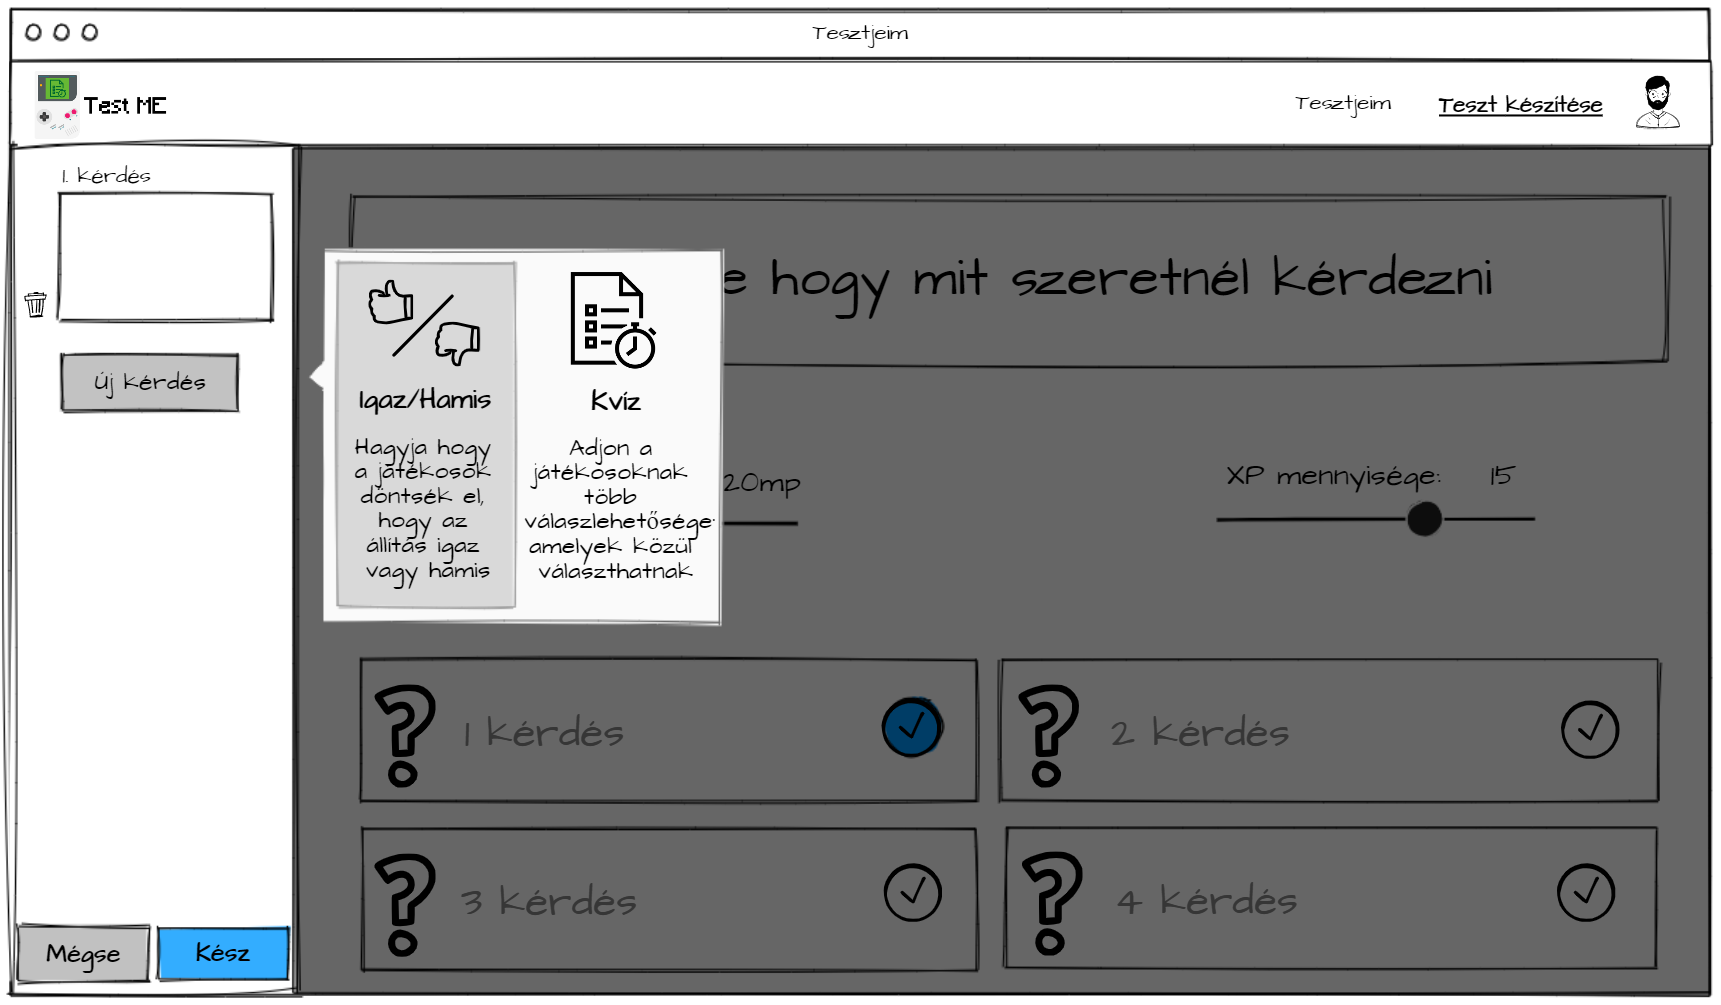
\includegraphics[width=\linewidth]{images/make_test2_wireframe.png}
    \caption{Új kérdés hozzáadása}
    \label{fig:new_question}
\end{figure}

Az igaz/hamis típusú kérdésnél csak annyi változik, hogy nem lehet válasz lehetőséget írni, csak egy állítást, amiről el kell dönteni, hogy valótlan vagy sem (\prettyref{fig:test_true_false}. ábra).

\begin{figure}[h!]
    \centering
    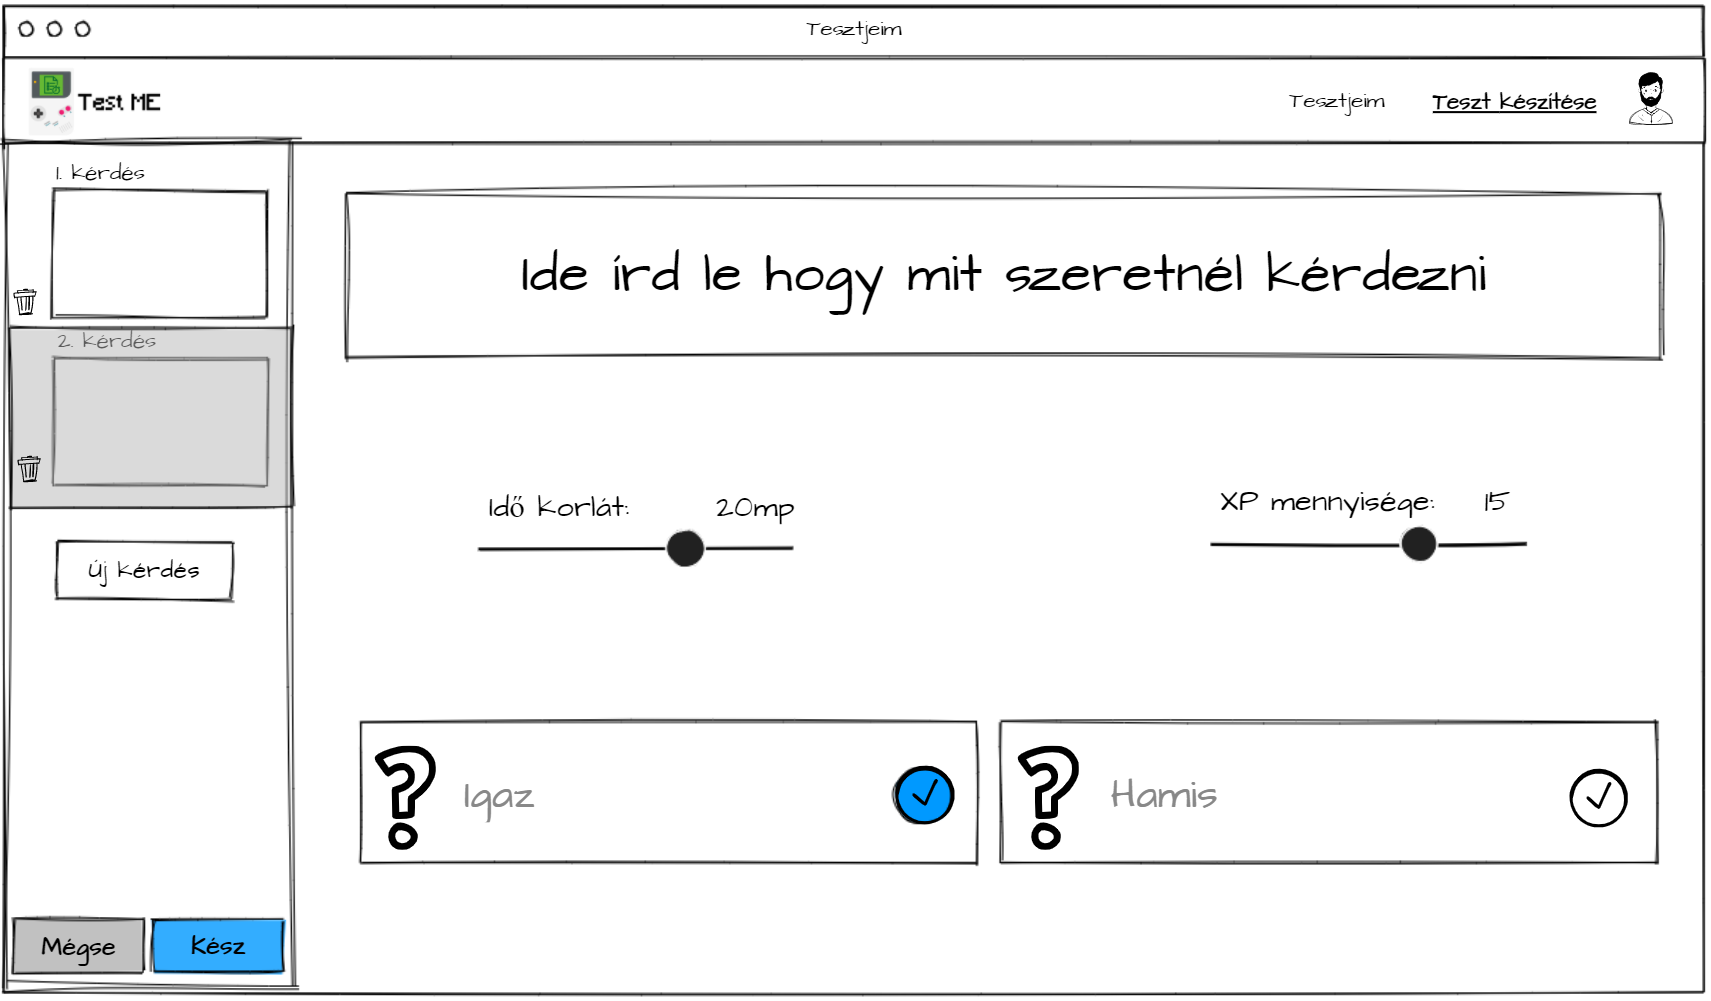
\includegraphics[width=\linewidth]{images/make_test3_wireframe.png}
    \caption{Igaz/hamis teszt készítése}
    \label{fig:test_true_false}
\end{figure}

Az utolsó lépés pedig az, hogy adunk címet a tesztnek, ilyen névvel fog megjelenni majd a tanulóknak. Ezután hozzáadunk tetszőleges számú diákot akiktől szeretnénk, hogy töltsék ki, egy kitöltési határidőt és elkészült a tesztünk (\prettyref{fig:save_test}. ábra).

\begin{figure}[h!]
    \centering
    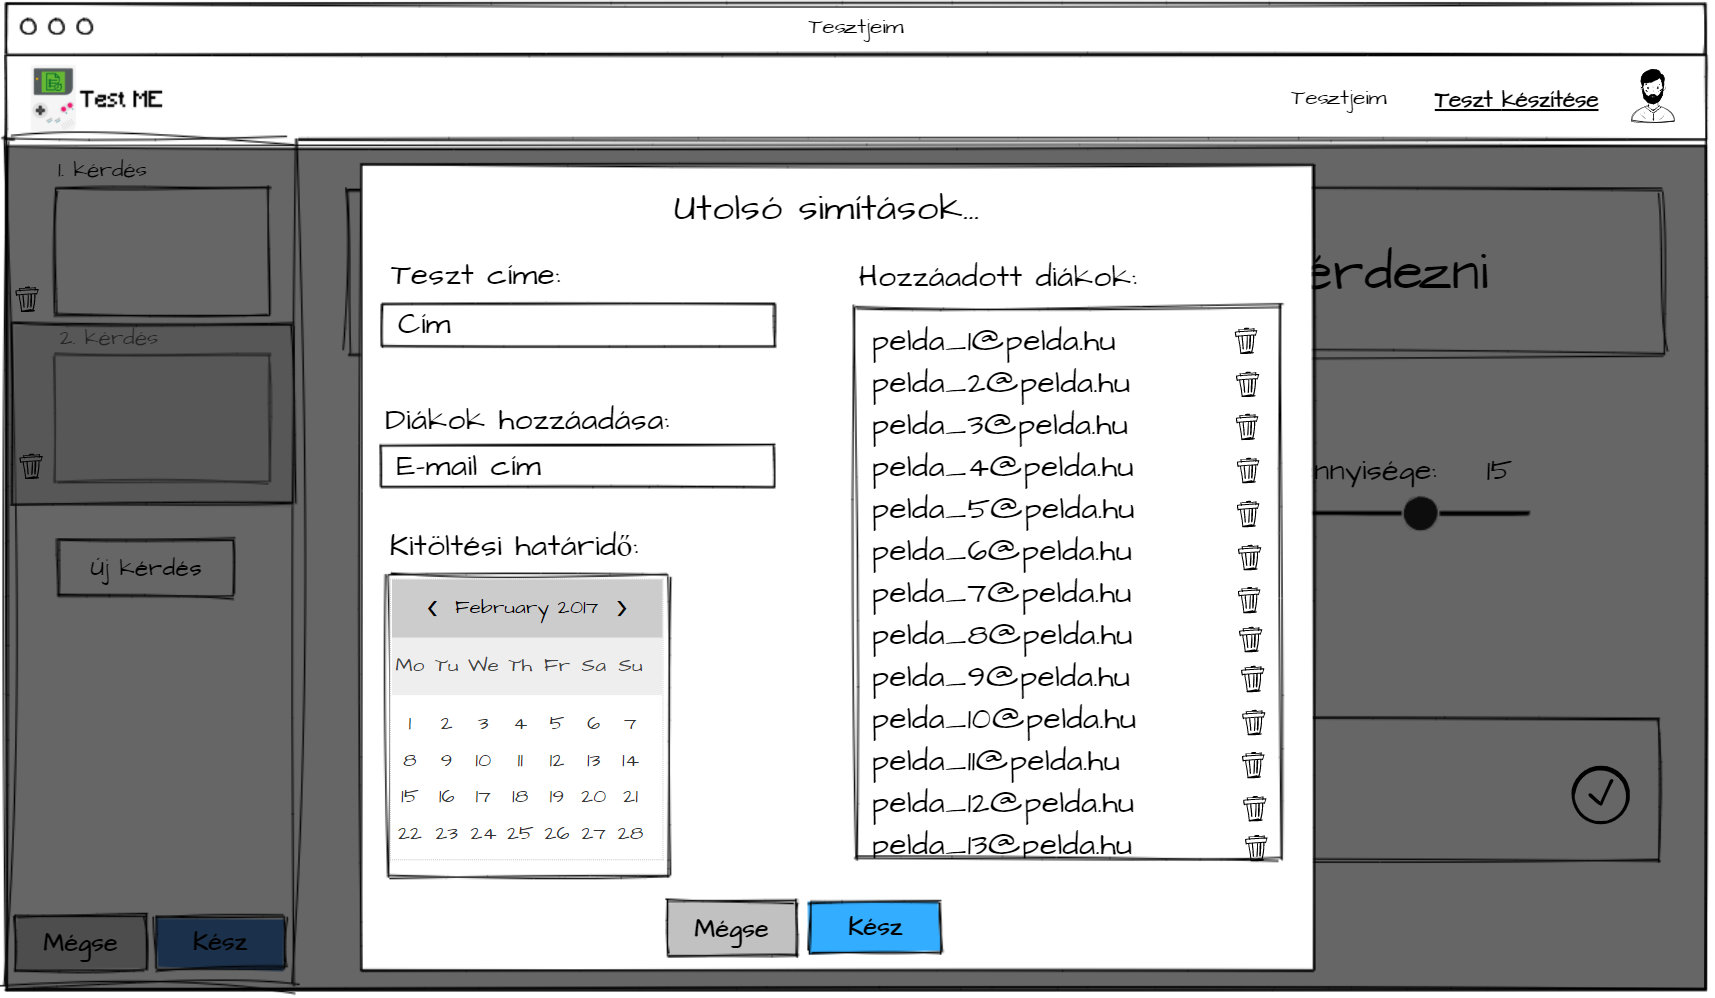
\includegraphics[width=\linewidth]{images/make_test4_wireframe.png}
    \caption{Adatok megadása és teszt elmentése}
    \label{fig:save_test}
\end{figure}

\SubSection{Saját tesztek}

\Aref{fig:my_tests}. ábrán a diákhoz rendelt teszteket látjuk. Itt azok az adatok láthatóak amiket tesztkészítéskor adtunk meg. Tehát a kitöltési határidő, a teszt címe, mennyi idő van rá, hány kérdés van és, hogy mennyi pontot lehet szerezni. Ezenkívül láthatjuk még, hogy mikor lett kiírva és egy kezdés gombot amivel kitölthetjük.

\begin{figure}[h!]
    \centering
    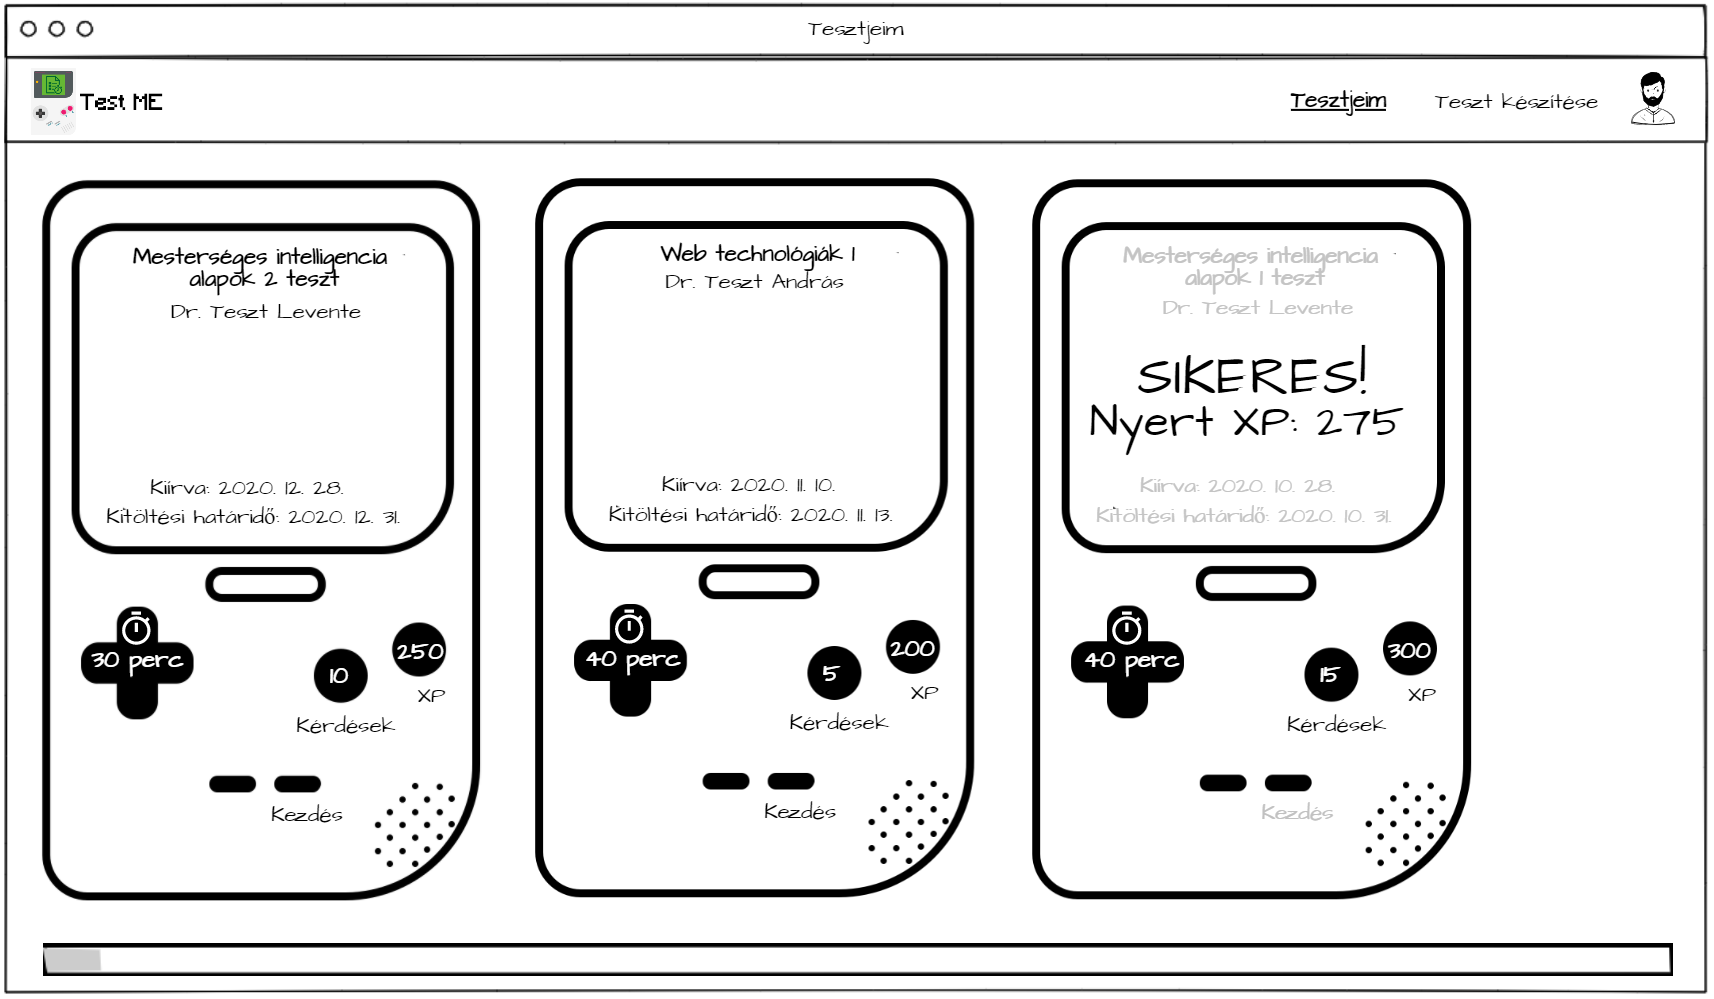
\includegraphics[width=\linewidth]{images/my_tests_wireframe.png}
    \caption{Felhasználóhoz rendelt tesztek}
    \label{fig:my_tests}
\end{figure}

\subsection{Teszt kitöltése}

Itt (\prettyref{fig:test_question}. ábra) egy kérdés látható teszt indítás után. Minden kérdésnél egy stopper órában láthatjuk, hány másodpercünk van még válaszolni.

\begin{figure}[h!]
    \centering
    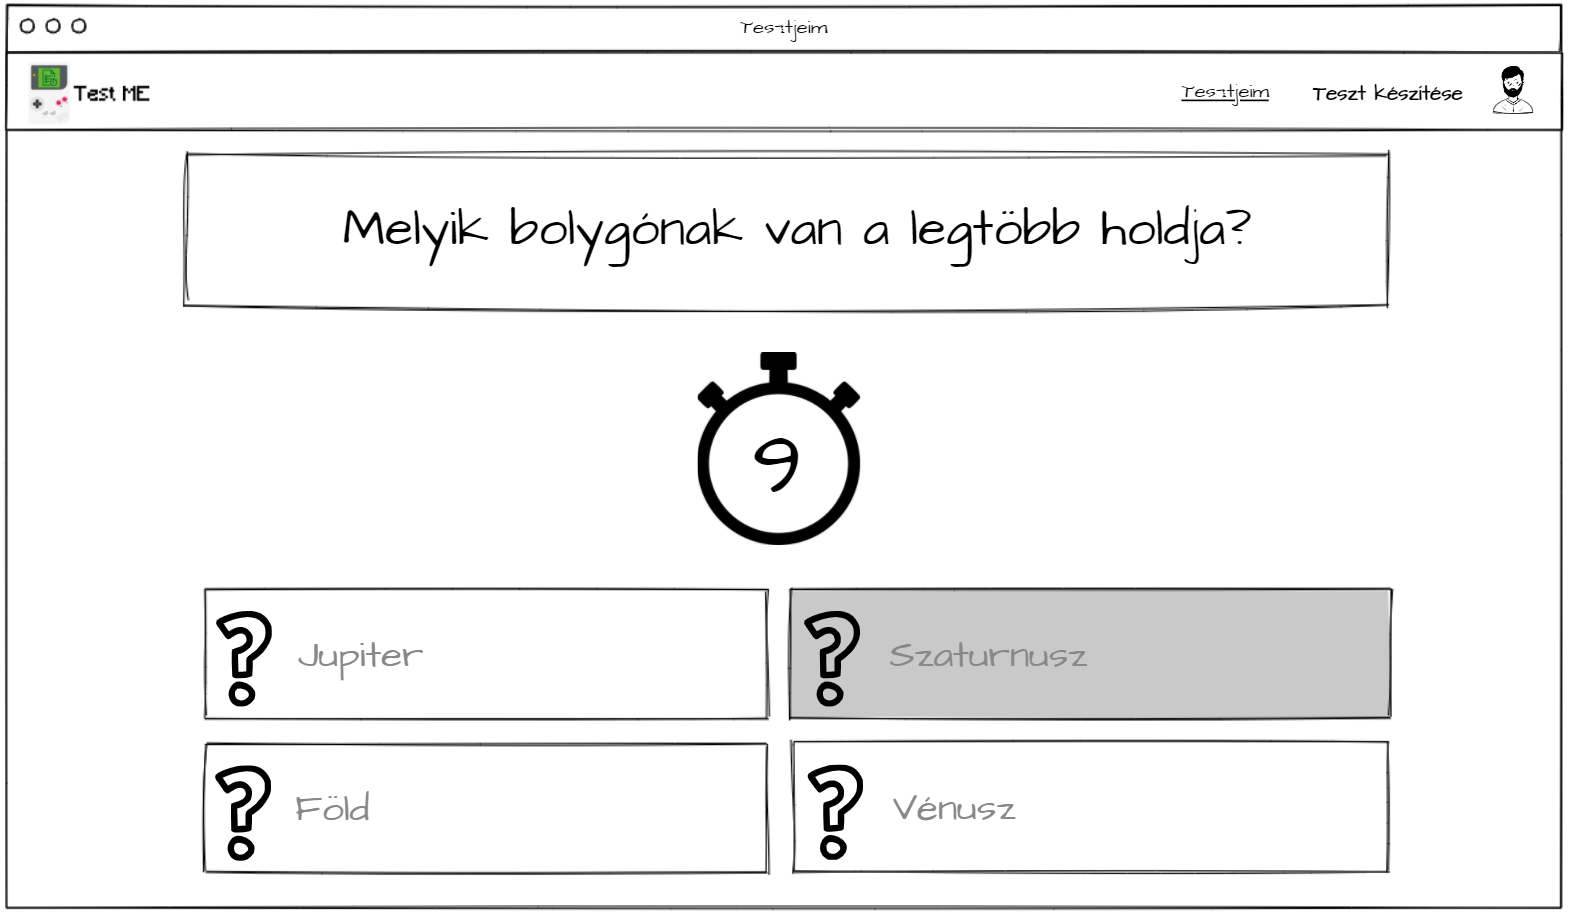
\includegraphics[width=\linewidth]{images/test1_wireframe.png}
    \caption{Feltett kérdés}
    \label{fig:test_question}
\end{figure}

Válaszadás után pedig láthatjuk, hogy ha válaszolunk egy kérdésre akkor melyik volt a jó (\prettyref{fig:test_answer}. ábra).

\begin{figure}[h!]
    \centering
    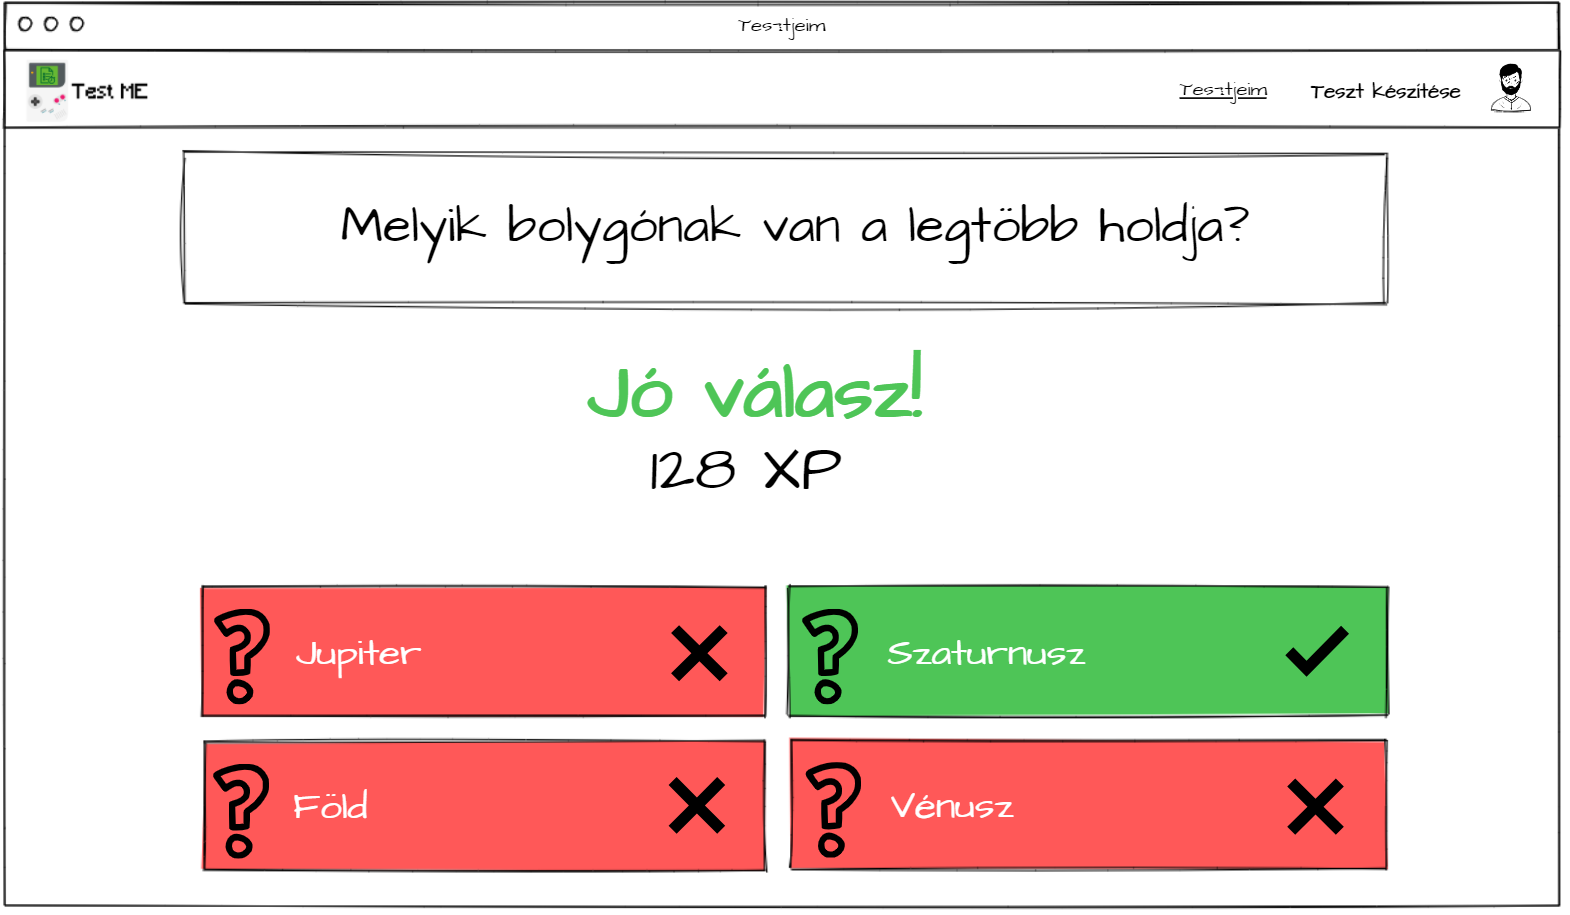
\includegraphics[width=\linewidth]{images/test2_wireframe.png}
    \caption{Válasz a kérdésre}
    \label{fig:test_answer}
\end{figure}

Miután válaszoltunk minden kérdésre, megnézhetjük mennyi pontot gyűjtöttünk és a kitöltők közül, kik lettek a legjobbak (\prettyref{fig:test_finished}. ábra).

\begin{figure}[h!]
    \centering
    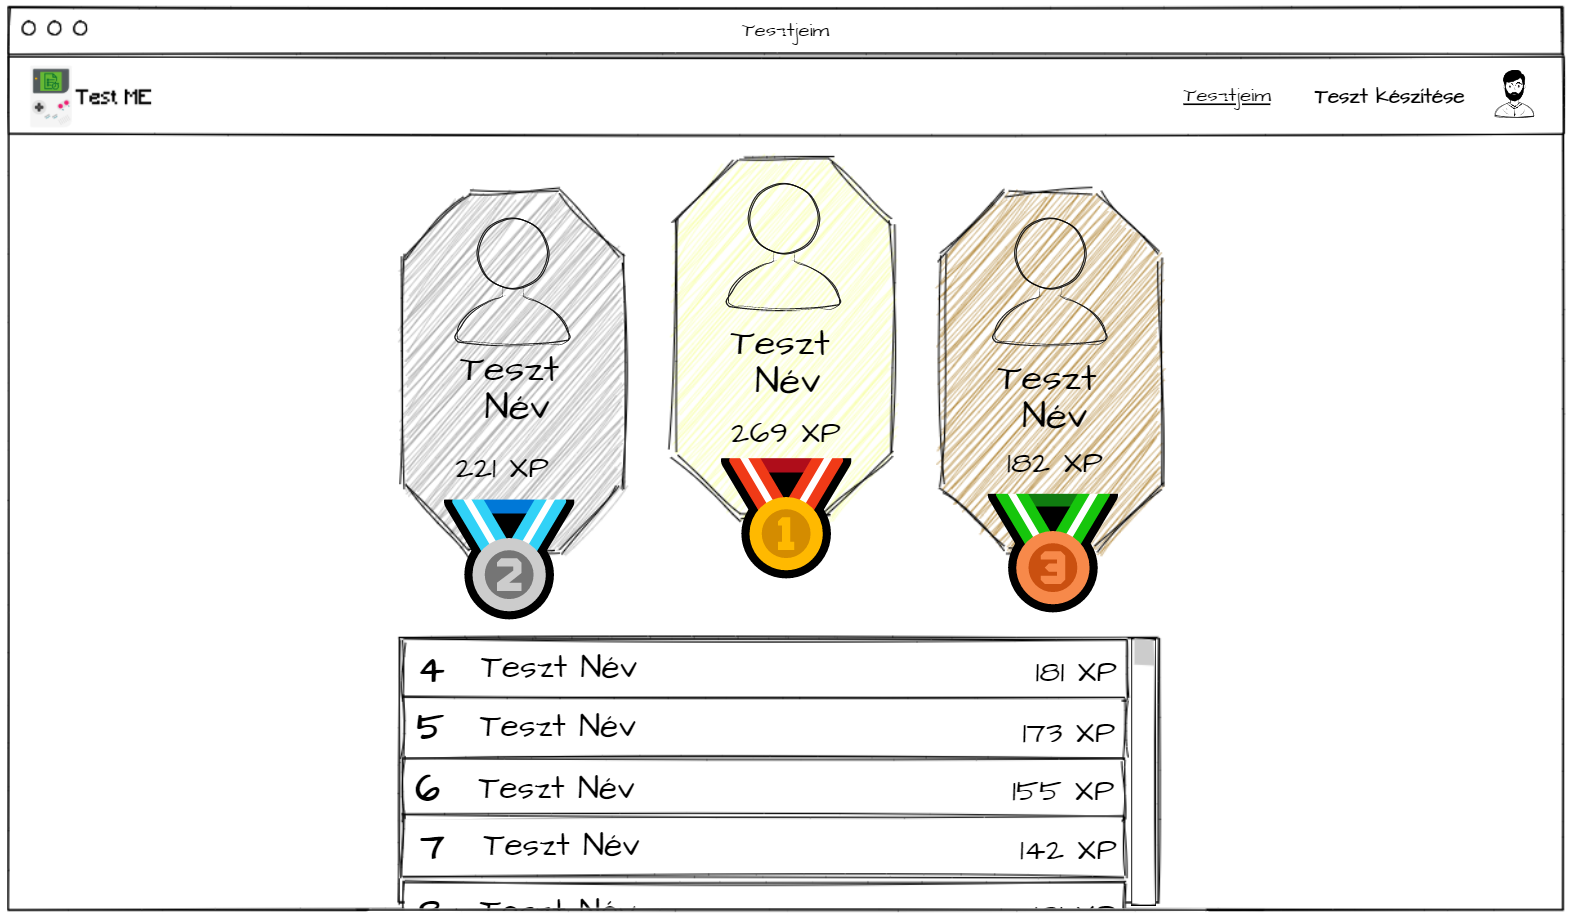
\includegraphics[width=\linewidth]{images/test3_wireframe.png}
    \caption{Teszt eredmény}
    \label{fig:test_finished}
\end{figure}

\Section{Az alkalmazás funkciói}

\begin{itemize}
    \item {Bejelentkezés/Regisztráció}
          \begin{addmargin}[\parindent]{0pt}
              Az oldalon lévő minden funkciót csak regisztráció vagy bejelentkezés után lehet használni. Ez azért fontos, hiszen csak így lehet a felhasználónak tesztet küldeni és kitöltés után hozzáadni a profiljához a pontokat és megjeleníteni a nevét a ranglistán. Az weboldal megnyitásakor a felhasználónak be kell jelentkeznie, egy helyes e-mail címmel és egy kellően biztonságos jelszóval vagy regisztrálnia kell, ha használni szeretné az oldalt.
          \end{addmargin}
    \item {Tesztkészítés}
          \begin{addmargin}[\parindent]{0pt}
              A Kahoot!-hoz hasonló teszt készítési felületet szeretnék létrehozni, ahol az elkészített teszteket hozzá lehet rendelni diákokhoz és ezután kitölthetik azokat.

              A két következő funkció a játékosítás alapját jelenti, viszont egy jó teszt nélkül értékét vesztik. A fejlődés és a teljesíteni vágyás a belső motiváció számunkra, hogy kihívásokat teljesítsünk. Viszont kihívások nélkül a pontok és a jelvények, vagy bármi féle jutalmak feleslegesnek tűnnek. Emiatt fontos, hogy a tesztek kellő kihívást nyújtsanak, hogy aztán a jó eredménnyel járó hasznokat is jutalomnak érezzük.
          \end{addmargin}
    \item {Pontgyűjtés}
          \begin{addmargin}[\parindent]{0pt}
              Minden regisztrált felhasználó rendelkezik majd egy szinttel és egy bizonyos pontszámmal, amelyet a tesztek kitöltésével szerezhetnek.
          \end{addmargin}
    \item {Ranglista}
          \begin{addmargin}[\parindent]{0pt}
              Ranglista a teszt teljes kitöltését követően alakul ki a legtöbbet szerzett pontok alapján.
          \end{addmargin}
    \item {Tesztek diákokhoz rendelése}
          \begin{addmargin}[\parindent]{0pt}
              Teszt létrehozása során email cím vagy valamilyen más egyedi azonosító segítségével hozzá lehetne rendelni diákokhoz a tesztet és így értesülnének róla, hogy ki kell tölteniük.
          \end{addmargin}
    \item {Összes hozzárendelt teszt megtekintése}
          \begin{addmargin}[\parindent]{0pt}
              Diákként meg lehet nézni az összes olyan tesztet amit valaki hozzá rendelt a profilhoz, és ezzel együtt a régiek eredményét is azért, hogy lássuk, hogy sikerült mindenkinek.
          \end{addmargin}
\end{itemize}

\Section{Adatmodell}
\label{Adatmodell}

Az adatokat egyed-kapcsolat diagrammon ábrázoltam, így a teljes kép könnyebben áttekinthető ezen rendszervázlat alapján.

\begin{figure}[H]
    \centering
    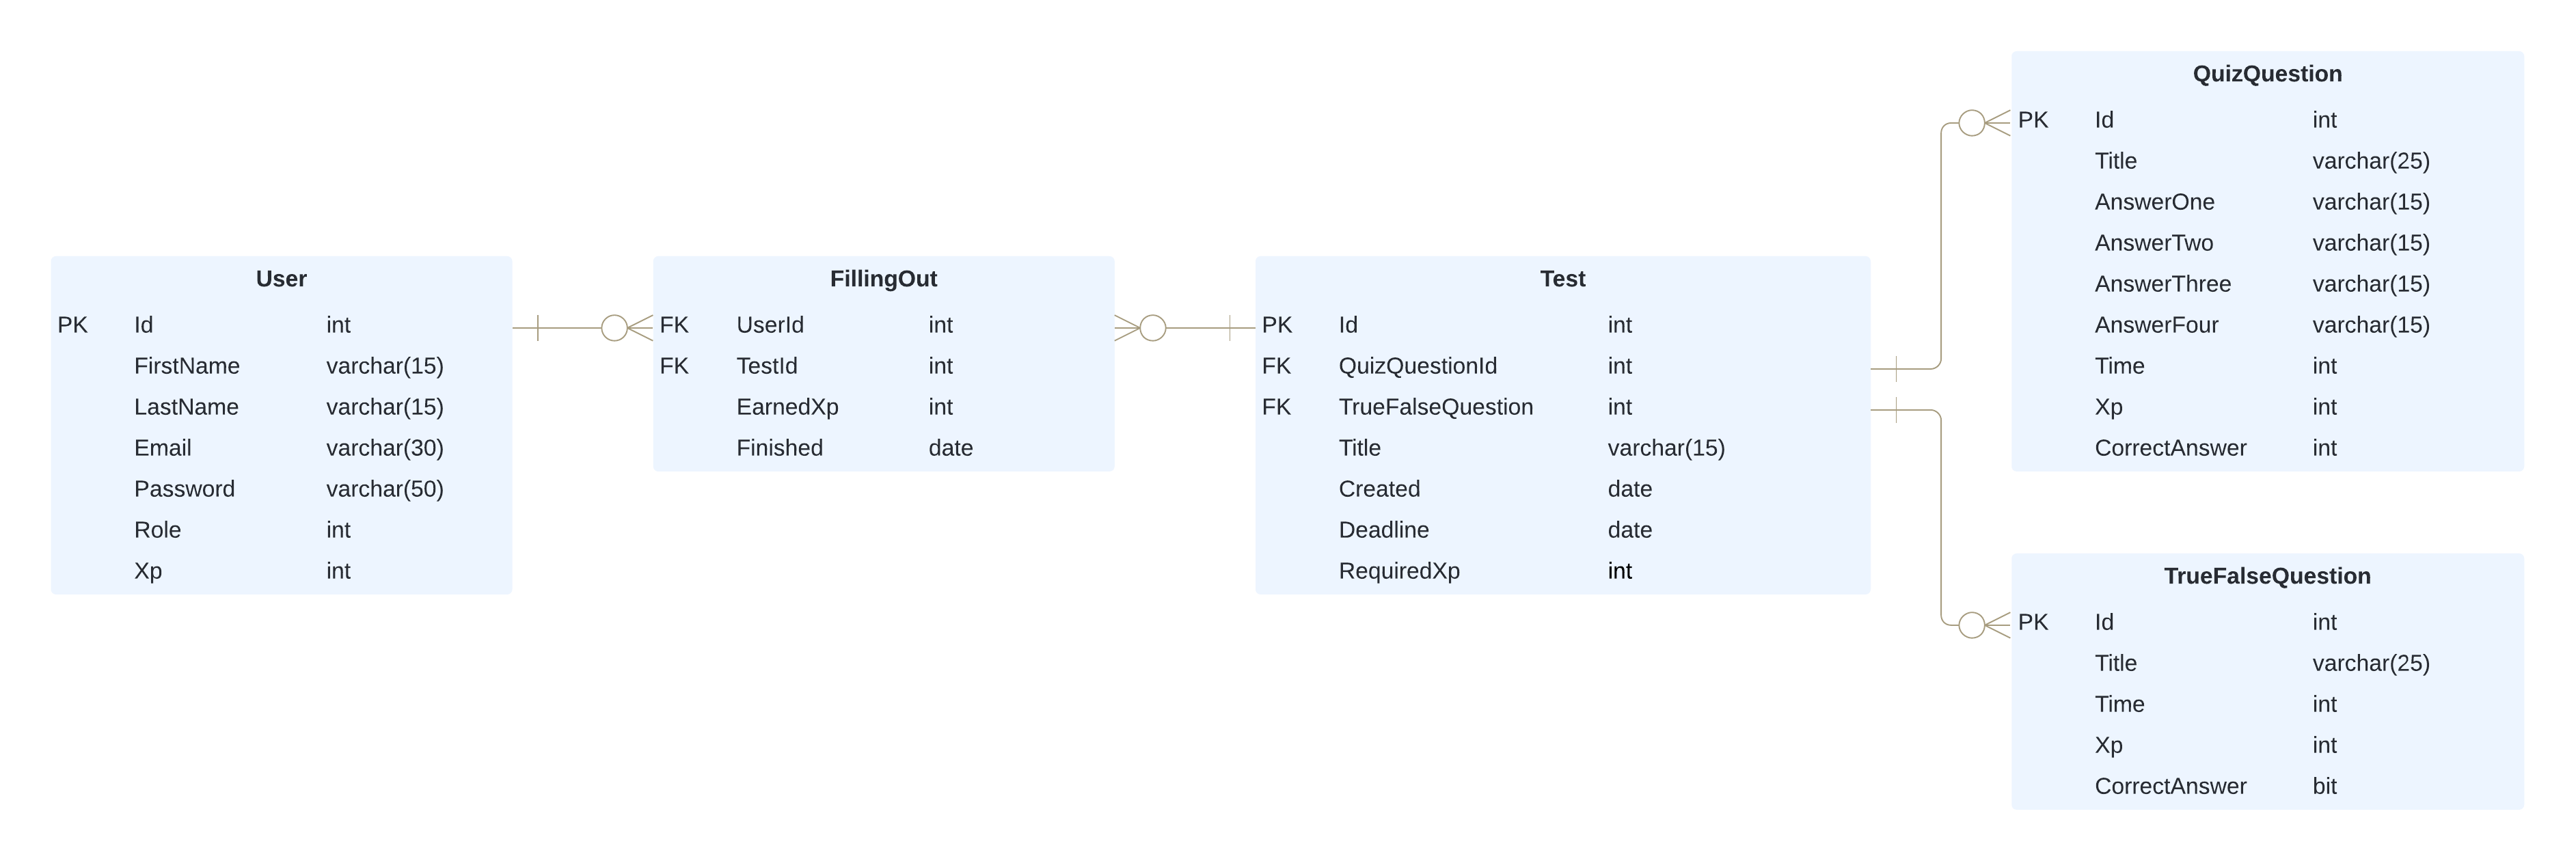
\includegraphics[width=\linewidth]{images/TestME_ER.png}
    \caption{ER modell}
    \label{fig:TestME_ER}
\end{figure}

A séma diagram (\prettyref{fig:TestME_ER}. ábra) az alábbi táblákat tartalmazza:
\begin{itemize}
    \item {User}
          \begin{addmargin}[\parindent]{0pt}
              Ez a tábla egy felhasználót reprezentál akinek az alap adatait bekérjük regisztrációkor. Ilyen például a keresztnév, vezetéknév, email cím, jelszó. Majd ezen felül még van regisztráció dátuma, és hogy visszaigazolta-e az e-mail címét. Valamint meg kell határoznia milyen szerepkörben szeretné használni az oldalt és miután töltött ki tesztet, növekedni fog az XP-je mennyisége így van egy XP adattag is.
          \end{addmargin}

    \item {Test}
          \begin{addmargin}[\parindent]{0pt}
              A \texttt{Test} tábla egy felhasználó által készített tesztet reprezentál. Egy teszten belül két típusú kérdés lehet: az egyik a kvíz, a másik az igaz/hamis. Ezen kívül benne van a teszt leírása, a készítő azonosítója, a teszt címe, hogy mikor készült, és hogy mi a kitöltési határidő.
          \end{addmargin}

    \item {Question}
          \begin{addmargin}[\parindent]{0pt}
              A \texttt{Question} egy kérdés adatait tárolja amibe beletartozik a kérdés szövege, a négy válasz, az idő, hogy mennyi pontot ér, és hogy melyik a helyes válasz.
          \end{addmargin}

    \item {UsersTest}
          \begin{addmargin}[\parindent]{0pt}
              Ez egy kapcsolótáblát képez a \texttt{Test} és a \texttt{User} tábla között. A kapcsolótábla azonosítója a két idegen kulcsból képzett összetett kulcs lesz. Tehát ebbe benne lesz a \texttt{Test} és \texttt{User} tábla idegen kulcsa. Valamint itt tárolódik el, hogy felhasználó kitöltötte már a tesztet és ha igen akkor mikor és mennyi pontot ért el. Ez a legtöbbet használt tábla az oldal működése során, hiszen innen szedjük ki az adatokat, ha megszeretnénk nézni milyen tesztjeink vannak és ha kitöltjük itt módosítjuk a pontot és a dátumot.
          \end{addmargin}

    \item {Answer}
          \begin{addmargin}[\parindent]{0pt}
              Ez a tábla egy kérdés válaszát tárolja el. Ebben benne van a kérdés és a \texttt{UsersTest} tábla \texttt{id}-ja, emellett, hogy meny idő alatt válaszolt a felhasználó a kérdésre és, hogy mi volt a válasza.
          \end{addmargin}
\end{itemize}

\Section{Az alkalmazás API-ja}
\label{API}

Az alábbi végpontokat (\textit{endpointokat}) szeretném használni az alkalmazásban:

\begin{itemize}
    \item \texttt{api/users}:
          \begin{addmargin}[\parindent]{0pt}
            Ezen az \textit{endpoint}-on tudunk majd lekérni egy felhasználót bejelentkezéskor, elmenteni és lekérni a felhasználó session-jét, az \texttt{id}-ját és az email címét. Valamint regisztrációkor ide szeretném elküldeni a felhasználó bejelentkezési adatait és azt, hogy ki szeretne jelentkezni.
          \end{addmargin}

    \item \texttt{api/tests}:
          \begin{addmargin}[\parindent]{0pt}
            Ha a diák ki akarja tölteni a tesztet, innen tudjuk majd lekérni a kérdésekkel együtt. Illetve, ha valaki készít egyet akkor ide lehet elküldeni az újat.
          \end{addmargin}

    \item \texttt{api/questions}:
          \begin{addmargin}[\parindent]{0pt}
            Egy teszthez tartozó kérdéseket külön kontroller kezeli és ide kerül majd elküldésre teszt létrehozáskor.
          \end{addmargin}
          
    \item \texttt{api/answers}:
        \begin{addmargin}[\parindent]{0pt}
            Teszt kitöltés után ide érkeznének a válaszok.
        \end{addmargin}
    
    \item \texttt{api/users-tests}:
          \begin{addmargin}[\parindent]{0pt}
            Ha egy diák meg akarja nézni a saját tesztjeit, hogy miket kell kitöltenie vagy miket töltött ki eddig, akkor azt innen tudjuk majd lekérdezni. Ezáltal kiírathatjuk őket a ,,Tesztjeim'' menüpont alatt, hogy befejezték-e már és mennyi pontot kaptak általa. Emellett a kitöltött és kitöltetlen tesztek száma is innen jön ami a főoldalon látható. Kitöltés után pedig itt kerül módosításra az \texttt{xp} adattag, a teszt után kapott pont alapján.
          \end{addmargin}
\end{itemize}
